\chapter{Introduction}
\label{ch:intro}
\hl{Intro to the first chapter
Give a nice history of solar observations and discuss current observing efforts as well as modeling efforts, but briefly; quickly move into atmosphere, corona}
\par The Sun is the most important celestial body to life on Earth. For the last five billion years, it has provided the light by which humans observe the world around them and the heat to save the planet from the frigid temperatures of interplanetary space. Because of its proximity, the Sun provides astronomers an exclusive and unique look into how stars behave. By observing and understanding the Sun, one can make conclusions about other types of stars in our galaxy and the universe.
%
\par Perhaps no other consistent celestial event has attracted as much attention as the solar eclipse. Solar eclipses have been observed and recorded for thousands of years, with some reports dating back to the fourteenth century BC \citep{golub_solar_2010}. The recordings of ancient eclipses have been heavily studied. Chinese rock drawings dating back to the Han dynasty (approximately 1900 years ago) appear to show the moon completely obscuring the Sun. Additionally, some have even suggested the Aubrey holes that surround the Stonehenge site were used to track and predict both solar and lunar eclipses \citep{golub_solar_2010}. Though some claims of ancient eclipse studies are controversial, it suffices to say that humans have long sought to study and explain the behavior of the nearest star to Earth.
%
\begin{figure}
	\centering
	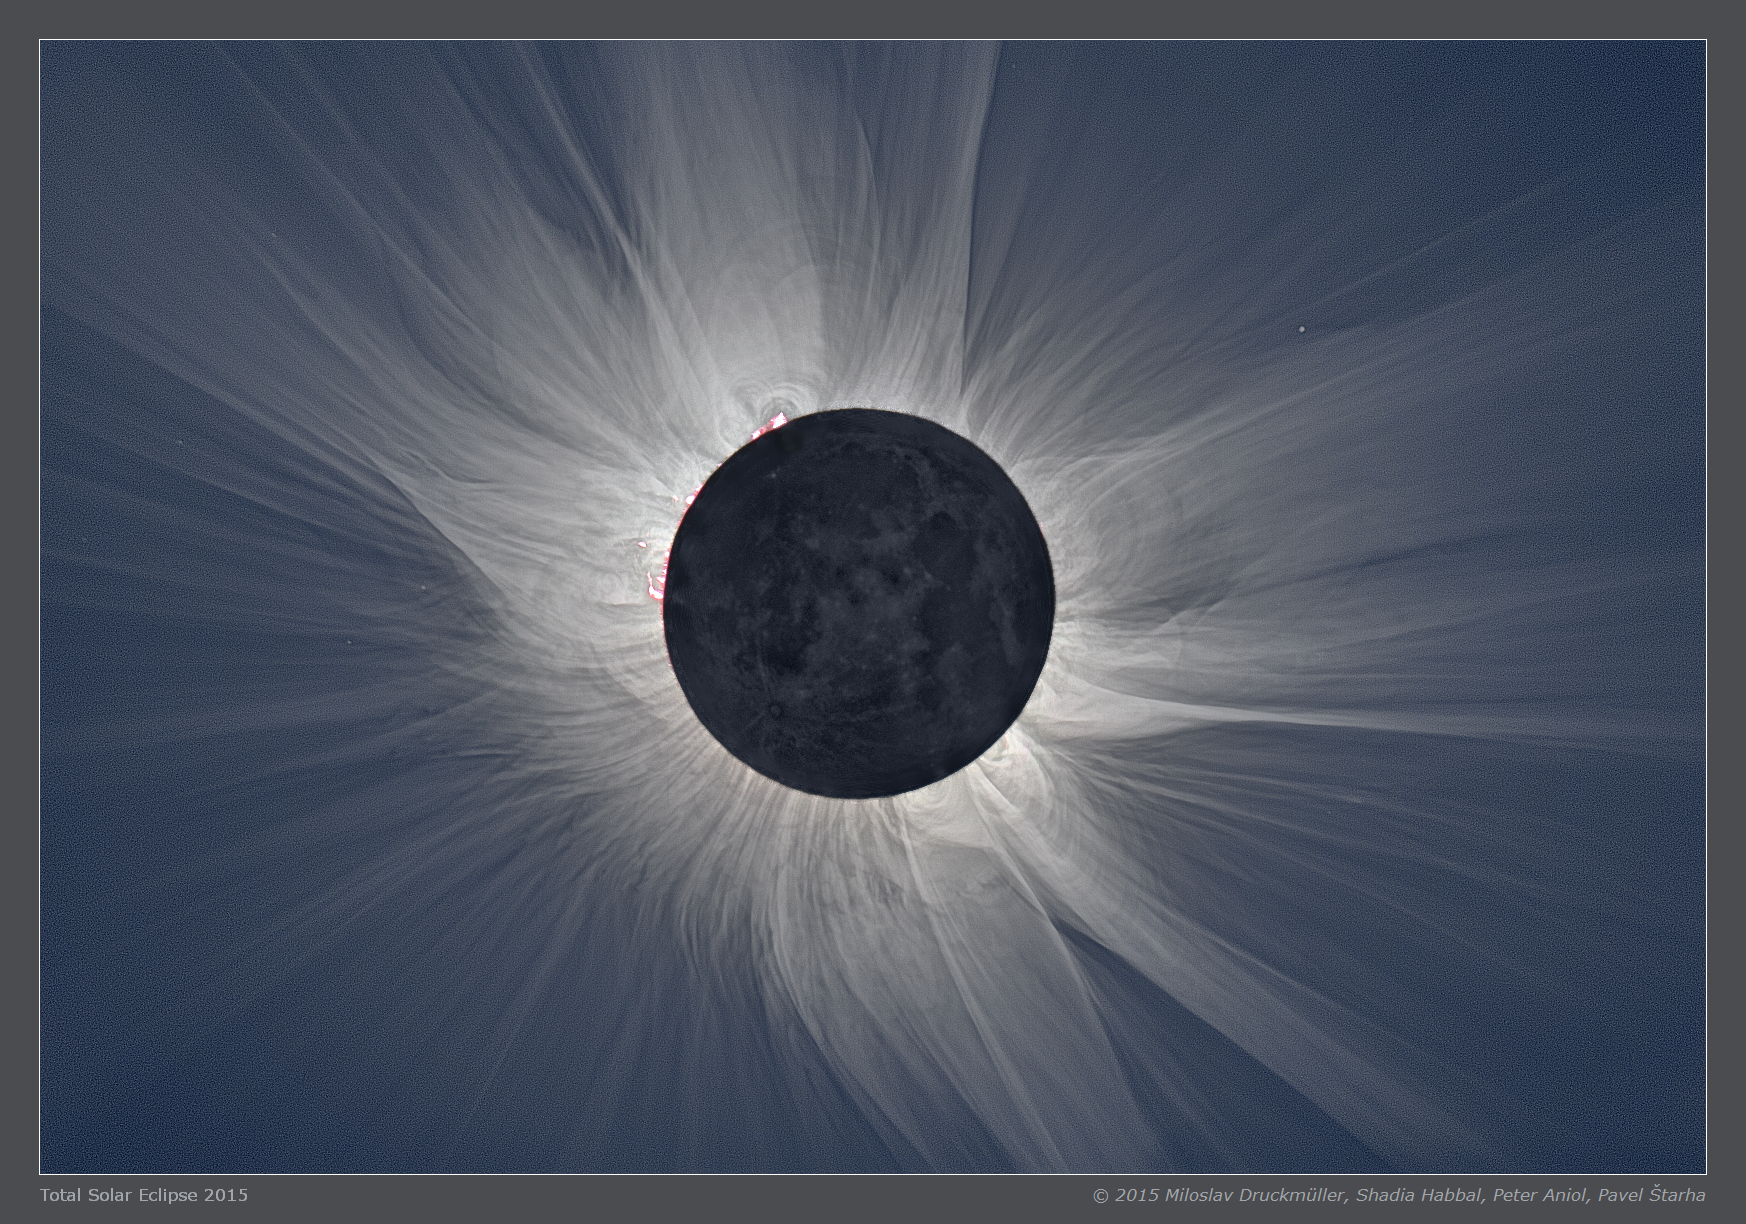
\includegraphics[width=0.7\textwidth]{figures/Tse_2015_Svalbard_800mm_Nikon_D810.png}
	\caption{Total eclipse as seen from Svalbard, Norway on March 20, 2015. Open and closed loops in the highly-structured solar corona are clearly visible. Photo courtesy of Miloslav Druckm\"{u}ller.}
	\label{fig:solar_eclipse}
\end{figure}
%
\par In particular, solar eclipses have captured the attention of artists for centuries. Cosmas Damian Asam, a Bavarian painter and architect active in the early eighteenth century, used images of solar eclipses in many of his works, including several frescoes and an altarpiece. \citet{olson_st._2007} discuss how Asam, a deeply religious artist, was commissioned several times to depict the vision of St. Gregory the Great, a Benedictine monk, as described in his work \textit{Dialogues}. 
%
\par One of these depictions, an altarpiece at a Benedictine monastery in Kladruby, Czech Republic (see Fig. 7 of \citet{olson_st._2007}), shows ``the visionary globe surrounded by a glowing halo of yellow light that more closely resembles the solar corona'' \citep{olson_st._2007}. An additional altarpiece at another monastery in Weltenburg, Germany shows a perhaps even more pronounced depiction of the solar corona during a total solar eclipse. \citet{olson_st._2007} note that, given his detailed depictions, Asam must have observed several solar eclipses as well as the solar corona, with these astronomical events profoundly impacting his depictions of supernatural events in his works. This is but one example of how solar eclipses and their consequential insight into the highly structured solar atmosphere, have shaped scientific and artistic discourse througout history.
%
%%
\section{Structure of the Solar Atmosphere}
\label{sec:structure}
\hl{This section will discuss the structure of the solar atmosphere including the different layers of the Sun and how they are connected. This will help to introduce the solar corona}
\par Though the Sun can be easily seen from Earth, its dynamic and highly structured atmosphere is not observable with the naked eye, with the one exception being brief glimpses of the corona during an eclipse. The interior of the Sun is of course very complex and constitutes a very different regime of physics than that seen in the solar atmosphere. Thus, this work will be primarily limited to the upper solar atmosphere with some discussion of the lower layers.
%
\par The solar atmosphere is often divided up into four separate regions: the photosphere, the chromosphere, the transition region, and the corona. Fig. \ref{fig:cartoon_layers} shows a cartoon of the different layers while Fig. \ref{fig:graph_layers} shows the density and temperature profiles of the atmosphere with each region labeled. The \textit{photosphere} is what we typically refer to as the solar surface, with the actual surface located where the optical depth, $\tau$, is equal to 1. This region also contains the lowest temperature on the Sun, approximately 4400 K, located about 525 km above the surface \citep{carroll_introduction_2007}. The photosphere is where the majority of the visibly (with the naked eye) observable photons originate.
%
\par The temperature minimum defines the top of the photosphere above which lies the \textit{chromosphere}. As can be seen from Fig. \ref{fig:graph_layers}, the density in the chromosphere is many orders of magnitude less than that of the photosphere and the temperature has increased from the minimum up to about $1\times10^4$ K. Though not visible with the naked eye, the chromosphere is highly structured. Structures such as spicules, tall columns of gas that extend high into the solar atmosphere thought to heavily impact the behavior of plasma in the corona \citep{de_pontieu_origins_2011}, originate in the photosphere as well as filaments, essentially spicules observed on-disk and plage, bright regions surrounding sunspots.
%
\begin{figure}
	\centering
	\subfigure[]{%
	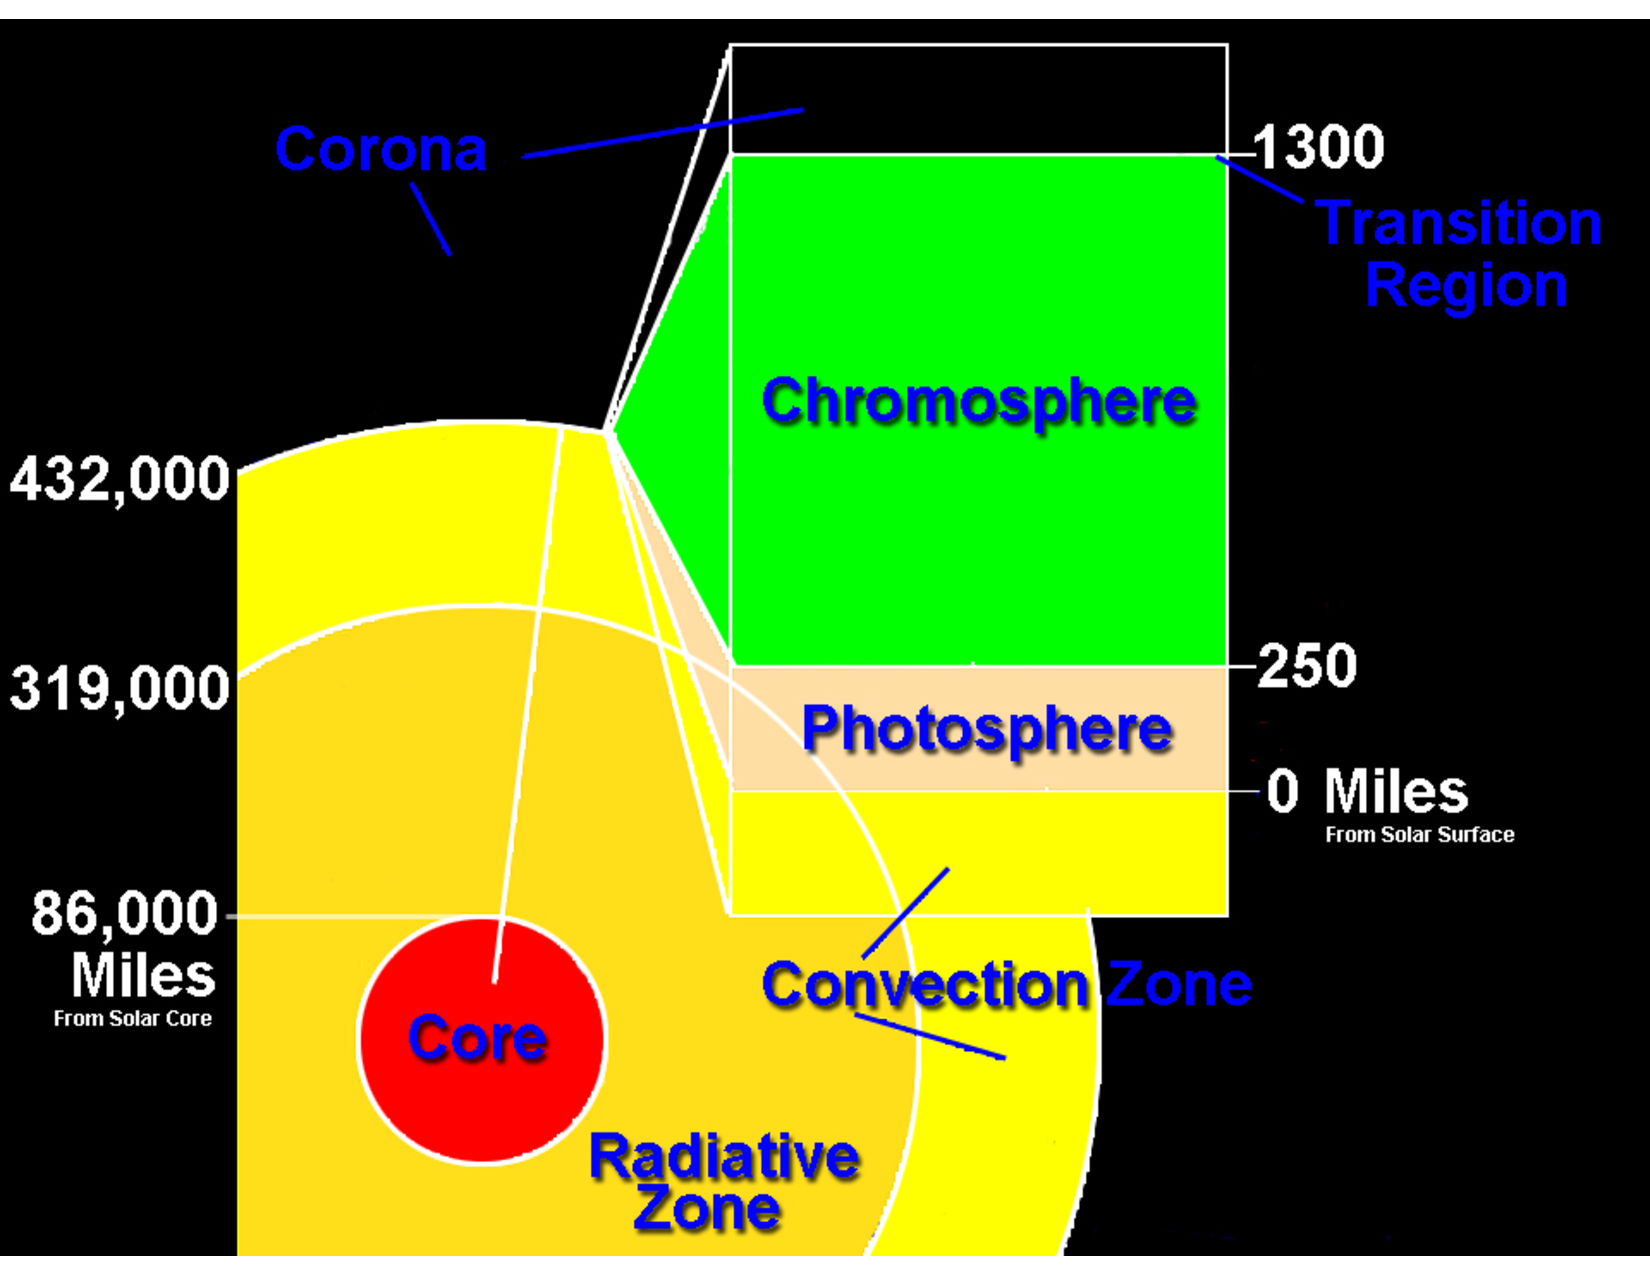
\includegraphics[width=0.45\textwidth]{figures/cartoon_layers.pdf}
	\label{fig:cartoon_layers}}
	\subfigure[]{%
	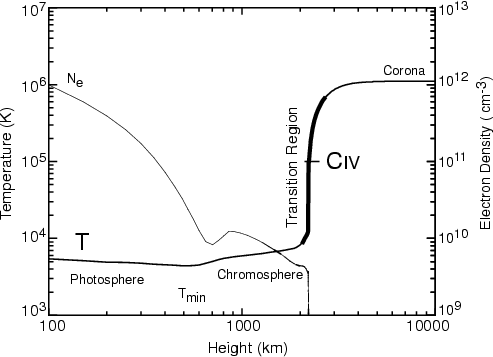
\includegraphics[width=0.45\textwidth]{figures/diagram_layers.png}
	\label{fig:graph_layers}}
	\caption{Layers of the solar atmosphere \textbf{(a)}Courtesy of NASA \textbf{(b)} Taken from \citet{gary_solar_2007}}
	\label{fig:layers}
\end{figure} 
%
\par Next is the \textit{transition region}, so called because of the steep temperature and density gradients (see Fig. \ref{fig:graph_layers}) that mark the transition between the chromosphere and the corona. The transition region is extremely thin, only a few hundred kilometers as compared to the chromosphere which extends over many thousands of kilometers. However, in this very short change in altitude, the temperature in the solar atmosphere jumps from $\approx1\times10^4$ K to temperatures exceeding $1\times10^5$ K. 
%
\par Finally, the solar \textit{corona}, or ``crown'', is the highly-dynamic uppermost layer of the Sun's atmosphere. Visible with the naked eye only during a total solar eclipse (see Fig. \ref{fig:solar_eclipse}), the corona is highly-structured and diffuse. Here, the temperature continues to increase, with typical coronal temperatures exceeding $1\times10^6$ K. Particularly high temperatures ($\approx1\times10^7$ K) have also been observed in \textit{active regions}, sites of intense magnetic activity associated with sunspots. These active regions can contain plasma as cool as $1\times10^4$ K as well and represent some of the most dynamic portions of the solar corona.
%
\par The work presented here will focus primarily on the plasma dynamics in the corona, in particular, in the cores of active regions where the intense magnetic field drives the motion of the plasma. In the following sections, we will discuss the origin of the solar magnetic field, its topology, how it impacts plasma in the solar corona, and finally how it connects to the anomalously high temperatures seen in the upper solar atmosphere.
%%
\section{The Solar Magnetic Field}
\label{sec:magnetic_field}
\hl{touch on field origin (dynamo theory), discuss how the field gets tangled, formation of loops, drives behavior of the atmosphere, lead into discussion of coronal heating, low beta versus high beta}
%
\section{The Coronal Heating Problem}
\label{sec:heating}
\hl{Here discuss coronal heating broadly, first evidence for high coronal temperatures, some proposed heating mechanisms, magnetic reconnection, AC versus DC heating, wave heating versus braiding etc.}
\section{Summary}
\label{sec:summary}
%
End with outline of the rest of the thesis: in ch. such and such we will discuss such and such